\section{Auswertung}

\subsection{Berechnung der Verdampfungswärme im niedrigen Druckbereich}

Mit der Apparatur \ref{fig:figskizze1} wurde im Versuch der Dampfdruck $p$ in $\si{\milli\bar}$ und die Temperatur $T$ in $\si{\celsius}$ gemessen. Die hergeleitete Lösung 
der Clausius-Clapeyron Differentialgleichung \eqref{eqn:wichtig} gibt Aufschluss auf die Verdampfungswärme $L$. Durch eine reziproke Darstellung der Temperaturen und eine Logarithmierung von beiden Seiten
ergibt sich folgender linearer Zusammenhang.

\begin{equation}
\label{eqn:1}
\text{ln}(p) = - \frac{L}{R} \cdot \frac{1}{T} + \text{ln}(p_{0})
\end{equation}
\\
In dieser Geradengleichung ist die Verdampfungswärme $L$ die Steigung und sie kann deshalb durch eine lineare Ausgleichsrechnung gewonnen werden.
Das p-T-Diagramm ist zunächst in Abbildung \ref{fig:plot1} geplottet, dabei wurden die Temperaturen in Kelvin umgerechnet.
\begin{figure}[h]
    \centering
    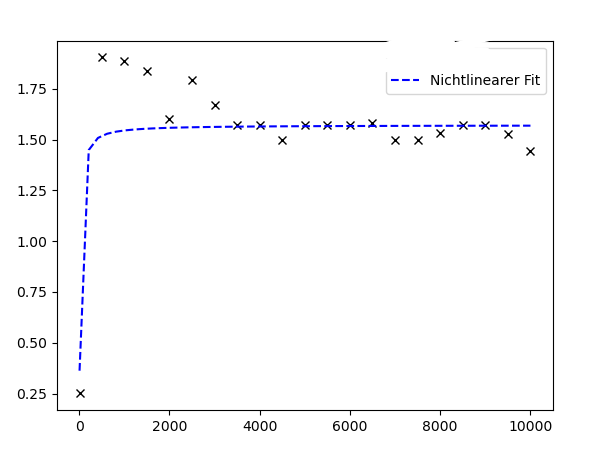
\includegraphics[width=\textwidth]{build/plot1.pdf}
    \caption{Gemessene Dampfdruckkurve bei niedrigen Drücken.}
    \label{fig:plot1}
  \end{figure}
Anschließend können durch Anpassung der Darstellung die Punkte in eine Geradengleichung überführt werden, wie in Gleichung \eqref{eqn:1} gezeigt. 
\\
Anhand einer lineare Regression, beispielsweise mit Python, kann eine Ausgleichsgerade durch die Punkte geplottet werden. Diese ist zusammen mit den Messpunkten in Abbildung \ref{fig:plot2} dargestellt.
\begin{figure}[h]
    \centering
    \includegraphics[width=\textwidth]{build/plot2.pdf}
    \caption{Linearer Fit durch die Messpunkte bei niedrigem Druck.}
    \label{fig:plot2}
\end{figure}
Die Ausgleichsgerade ist von der Form

\begin{equation}
\text{ln}(p) = a \cdot \left( \frac{1}{T}\right) +b
\end{equation}
\\
und die folgenden Parameter ergeben sich.
\begin{align}
a &= \SI{-4710.774(43656)}{\kelvin} \\
b &= \SI{19.492(0133)}{}
\end{align}
Aus dem bereits zuvor genannten Zusammenhang \eqref{eqn:1} folgt nun sofort.

\begin{equation}
a = -\frac{L}{R} \quad \to \quad L = -R \cdot a
\end{equation}
\\
Die universelle Gaskonstante $R$ ist eine exakte Größe und lässt sich der Literatur \cite{Naturkonstanten} entnehmen.
Für die Verdampfungswärme $L$ ergibt sich letztendlich.
\begin{equation}
L = \SI{39.168(0363)}{\kilo\joule\per\mol\per\kelvin}
\end{equation}
Der Fehler auf die Verdampfungswärme entspringt aus der folgenden Gaußschen Fehlerfortpflanzung. Diese ist hier besonders simpel auf Grund des linearen Zusammenhangs zwischen $a$ und $L$. 
\begin{equation}
\increment L = -R \cdot \increment a
\end{equation}

Um festzustellen wie viel Arbeit aufgebracht werden muss, um die Anziehungskräfte der restlichen Moleküle zu überwinden,
kann mit der allgemeinem Gasgleichung die Verdampfungswärme $L$ angenähert werden.
Dazu wird, auf Grund der Dimension, die Gleichung \eqref{eqn:gas} auf [$\si{\joule}/\si{\mol}$] angepasst und entsprechend gekürzt.
\begin{equation}
    \left[\frac{\si{\bar\meter\tothe{3}}}{\si{\mol}}=\frac{\si{\joule}}{\si{\mol\kelvin}}\si{\kelvin}\right]
\end{equation}
Mit der gegebenen Temperatur erschließt sich ein Wert von $3101\si{\joule\per\mol}$ für $L_a$. Die Differenz folgt.
\begin{align*}
    L_i&=L-L_a \hspace{1cm}  | L = \SI{39.168(0363)}{\kilo\joule\per\mol\per\kelvin} \\
    L_i&= \SI{36.067(0363)}{\kilo\joule\per\mol\per\kelvin}
\end{align*}
Um ein Ergbenis pro Molekül zu bekommen gilt es nun $L_i$ durch den für ein $\si{\mol}$ definierten Wert zu teilen.
In Elektronenvolt umgeformt beträgt die Verdampfungswärme.
\begin{equation}    
    L_i= \SI{0.406(0003)}{eV}
\end{equation}

\subsection{Berechnung der Verdampfungswärme im hohen Druckbereich}

Analog zu der vorherigen Auswertung kann hier die Verdampfungswärme $L$ für die ermittelte Dampfdruckkurve im zweiten Teil des Versuchs \ref{fig:figskizze2} errechnet werden.
Die Dampfdruckkurve ist zunächst in Abbildung \ref{fig:plot3} dargestellt.
\begin{figure}[h]
    \centering
    \includegraphics[width=\textwidth]{build/plot3.pdf}
    \caption{Gemessene Dampfdruckkurve bei höheren Drücken.}
    \label{fig:plot3}
\end{figure}
Wie zuvor wird die Darstellung durch Logarithmierung angepasst und eine Ausgleichsgerade ermittelt. Das Ergebnis ist in Diagramm \ref{fig:plot4} abgebildet.
\begin{figure}[h]
    \centering
    \includegraphics[width=\textwidth]{build/plot4.pdf}
    \caption{Linearer Fit durch die Messpunkte bei hohem Druck.}
    \label{fig:plot4}
\end{figure}
Die Parameter der Ausgleichsgeraden lauten hier wie folgt.
\begin{align}
    a &= \SI{-6164.084(16549)}{\kelvin} \\
    b &= \SI{15.905(0384)}{}
\end{align}
Durch den erneuten Vergleich mit Gleichung \eqref{eqn:1} lässt sich nun wieder die Verdampfungswärme $L$ finden.
\begin{equation}
L = \SI{51.251(1375)}{\kilo\joule\per\mol\per\kelvin}
\end{equation}
\\
Zusätzlich kann hier noch die Verdampfungswärme in Abhängigkeit von der Temperatur ermittelt werden. Dazu wird die Clausius-Clapeyronsche
Differentialgleichung \eqref{eqn:dgl} zunächst nach $L$ aufgelöst.

\begin{equation}
    \label{eqn:lol}
L = (V_{D}-V_{F})T \cdot \frac{\text{d}p}{\text{d}T}
\end{equation}
Hier kann nun wieder die Annahme $V_{F} = 0$ wie bei der Lösung der Differentialgleichung verwendet werden. Das Volumen $V_{D}$ lässt sich nun allerdings wie zuvor erwähnt nicht mehr
durch die allgemeine Gasgleichung bestimmen. Hier gilt die folgende Annäherung.
\begin{equation}
\left( p + \frac{a}{V^{2}}V = R \cdot T \right)
\end{equation}
Die Lösung für $V$ folgt dann als Lösung des Polynom zweiten Grades und sie kann direkt in die Gleichung \eqref{eqn:lol} eingesetzt werden.
\begin{equation}
L = \left(\frac{RT}{2p} \pm \sqrt{\left( \frac{RT}{2p}\right)^2 -\frac{a}{p}}\right) T \cdot \frac{\text{d}p}{\text{d}T}
\end{equation}
Der Druck $p$ sowie der auftretende Differentialquotient $\text{d}p$/$\text{d}T$ kann durch ein Polynom dritten Grades bestimmt werden. Dazu wird ein
Fit durch die gemessenen Punkte gelegt. Das Polynom hat dann die folgende Form.
\begin{equation}
p(T) = AT^{3} + BT^{2} + CT + D
\end{equation}
Die passenden Parameter lauten.
\begin{align*}
    A &= \SI{0.000010(2)}{\bar\per\kelvin\tothe{3}} \\
    B &= \SI{-0.002939 (952)}{\bar\per\kelvin\tothe{2}} \\
    C &= \SI{0.365120 (150603)}{\bar\per\kelvin}\\
    D &=  \SI{-17.336223 (7844842)}{\bar} \\
\end{align*}
Nun kann das Polynom noch abgeleitet werden